%!TEX root = ../thesis.tex
\chapter{Introduction}
\label{introduction}
One of the most important factors for the success of an Information Technology (IT) company is its \Quote{way of working}: a set of rules that make systematic, disciplined and quantifiable the activities of the project.
In time these could become \textit{best practices}, i.e. a well known to work way of working that is reliable and has demonstrated to have succeeded.\\
To correctly apply these rules and follow the work of its employees, the company has to use software instruments, which, in the context of this thesis, are Jira and Confluence.

\section{Premise}
	This document is a report of the two month curricular internship done between June and July 2019 at Athonet under the supervision of Dott. Fabio Giust.
	It contains a description of the work that done and an introduction to Agile and Scrum software developing methodologies.\\
	To introduce and describe some of the arguments there will be a few comic strips of \Quote{Dilbert}, a character invented by Scott Adams\cite{dilbert}.
	It satirically represents the problems that can be present in any small or big IT company.
	\begin{figure}[H]
		\centering
		
\includegraphics[width=1\textwidth]{resources/Dissertate}\\
		\caption[Dilbert, \Quote{Plan A}]{Dilbert, \Quote{Plan A}}
	\end{figure}
	The \Quote{Glossary} section at the end of the document describes technical words that would need a more specific introduction: these are marked as \gls{Example}.\\
	
\section{The company}
	Athonet\cite{athonet} is a telecommunication company headquartered nearby Vicenza, Italy.
	It stem from the idea that \gls{broadband networking}\glsadd{Broadband networking} should be easily available to people in rural areas and to companies that work in mission critical services or special environments like shipping, mining companies or even hospitals (safety critical).\\
	Officially it was founded in 2004, although a working prototype of their idea was already developed by the CEO (Chief Executive Officer) and CTO (Chief Technology Officer) that were working alongside in Ericsson\cite{ericsson} at that time.
	\begin{figure}[H]
		\centering
		
\includegraphics[width=.7\textwidth]{resources/ath_logo}\\
		\caption[Athonet's logo]{Athonet's logo}
	\end{figure}
	\gls{Low latency}\glsadd{Low latency} communication, reliability and security are at the core of what Athonet provides.
	Their main product is \Quote{PriMo}, a device that allows to create a dedicated \gls{core network}\glsadd{Core network}, or enterprise \gls{LTE}\glsadd{LTE}.
	\begin{figure}[H]
		\centering
		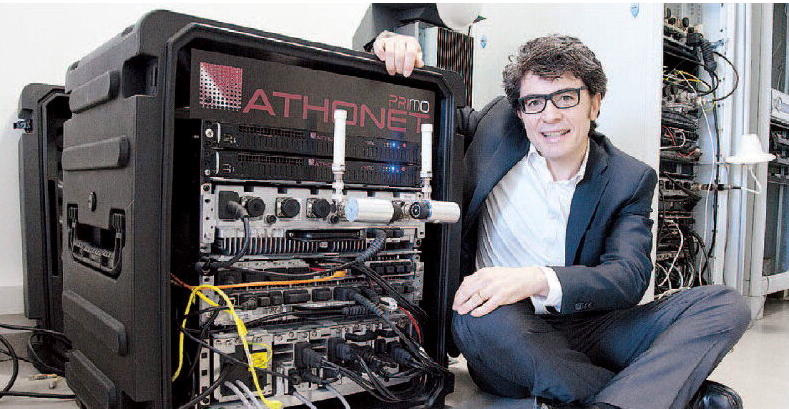
\includegraphics[width=.5\textwidth]{resources/gianluca_primo}\\
		\caption[]{Athonet's main product \textbf{\Quote{PriMo}}\cite{gianluca_primo}}
	\end{figure}
	The philosophy behind PriMo is that \Quote{the software is the network}, as Athonet was a pioneer in decoupling the software from the hardware, in order to have the solution running on different general purpose computing hardware, e.g., based on x86 processors.\\
	In 2012, after a disastrous earthquake destroyed all the communication lines in Emilia Romagna, Athonet has reestablished connectivity, thus showing the how PriMo can be used on the field in emergency situations.\\
	Athonet installed PriMo at the top of a school, allowing them to cover the affected area not only for the operators of Servizio Civile but for the citizens as well.\\
	In December 2013, Athonet has been rewarded by Giorgio Napolitano, the then President of the Italian Republic, with a medal for merits for the sustainability in the digital sector\cite{athonet_presidente}.\\
	Lately they have migrated some of their functions to the cloud: by using AWS they have achieved a hybrid product, BubbleCloud, a plug and play solution that allows to locally deploy the physical Edge Nodes while managing them from the AWS cloud.\\
	This small business has much to offer, considering that some of it's competitors are giants like Nokia and Ericsson.\\
	As a proof of the continuous will to improve and for the solution it provides, Athonet has been awarded with four Global Mobile Awards at the GSMA Mobile World Congress, held in February 2019 in Barcelona\cite{athonet_premi}.

\section{The project}
	It consists in installing and configuring two main software tools, \textbf{Jira} and \textbf{Confluence}, alongside plugins to add more functions and enhance their potentiality.
	However, the most important part of this project is not installing the software, but adapting it to the needs of the company.\\
	As said earlier Athonet is a growing business, and because of this it needs to give itself some internal rules and specifications to follow when working on a task, communicating with the client or even share internal information to employees.
	Not only for themselves but for clients they work with as well, since most big companies require that their partners have internal regulations, no matter the number of people in the company.\\
	As will be explained in the following chapters, Jira is an Issue Tracking System (ITS), a software that allows to follow and record tasks (like resolving bugs or implementing features), called issues, that are related to a project, while Confluence is a software for sharing knowledge, that means exchanging internal documents, keeping a wiki, having documentation available and even for customers, etc.\\
	The assignment was to demonstrate that these tools are what Athonet needs to be a stronger an coherent company, in which information is always shared and available, while maintaining a history of changes, by creating an environment that suited their needs and that can evolve alongside the company.\\
	To do this I have learned the basics of Agile and Scrum methodologies, how a company operates internally and with their clients and how introducing a new tool may improve the way of working, even if it creates chaos at the beginning.

\section{Document organization}
	The main part of this thesis is organized as follows:
	\begin{itemize}
		\item \Chapref{introduction} or \Quote{Introduction}: describes the overall content of this document
		\item \Chapref{chapter_2} or \Quote{The internship project}: describes in detail the objectives and planning of the internship project
		\item \Chapref{chapter_3} Chapter 3 or \Quote{Agile processes and methodologies}: an introduction to the Agile software development
		\item \Chapref{chapter_4} or \Quote{Jira and Confluence: the essentials}: describes the most valuable functionalities of Jira and Confluence
		\item \Chapref{chapter_5} or \Quote{Project implementation}: details how the project has been implemented by dividing it into time periods
		\item \Chapref{conclusions} or \Quote{Conclusions}: contains the retrospective of the project, future developments and personal considerations
	\end{itemize}
	
